%% LyX 2.3.2 created this file.  For more info, see http://www.lyx.org/.
%% Do not edit unless you really know what you are doing.
\documentclass[11pt]{article}
\usepackage[LGR,T1]{fontenc}
\usepackage[latin9]{inputenc}
\usepackage{geometry}
\geometry{verbose,tmargin=1in,bmargin=1in,lmargin=1in,rmargin=1in}
\usepackage{color}
\usepackage{amsmath}
\usepackage{amssymb}
\usepackage{graphicx}
\usepackage{setspace}
\doublespacing
\usepackage[unicode=true,
 bookmarks=false,
 breaklinks=false,pdfborder={0 0 1},backref=section,colorlinks=true]
 {hyperref}
\hypersetup{pdftitle={Terra Money White Paper},
 linkcolor=black,citecolor=blue,filecolor=magenta,urlcolor=blue}

\makeatletter

%%%%%%%%%%%%%%%%%%%%%%%%%%%%%% LyX specific LaTeX commands.
\DeclareRobustCommand{\greektext}{%
  \fontencoding{LGR}\selectfont\def\encodingdefault{LGR}}
\DeclareRobustCommand{\textgreek}[1]{\leavevmode{\greektext #1}}
\ProvideTextCommand{\~}{LGR}[1]{\char126#1}


%%%%%%%%%%%%%%%%%%%%%%%%%%%%%% User specified LaTeX commands.
\usepackage{xcolor}
 \usepackage{adjustbox}
\usepackage{titling}\usepackage{titlesec}\usepackage{eurosym}
\usepackage{harvard}\usepackage{amsfonts}
\usepackage{pdflscape}\usepackage{chicago}\setcounter{MaxMatrixCols}{30}
\usepackage[bottom]{footmisc}


% This shrinks the space before and after display formulas
\usepackage{etoolbox}
\apptocmd\normalsize{%
\abovedisplayskip=5pt
%\abovedisplayshortskip=6pt % plus 3pt
 \belowdisplayskip=6pt
 %\belowdisplayshortskip=7pt plus 3pt
}{}{}

% slim white space before title, section/subsection headers
\setlength{\droptitle}{-.75in}
\titlespacing*{\section}{0pt}{.2cm}{0pt}
\titlespacing*{\subsection}{0pt}{.2cm}{0pt}
\definecolor{mygray}{gray}{0.95}

\makeatother

\usepackage{listings}
\lstset{language=C,
basicstyle={\ttfamily},
backgroundcolor={\color{mygray}},
keywordstyle={\color{black}\bfseries},
frame=tlrb}
\begin{document}
\title{Terra Money:\\
 Stability and Adoption}
\author{Evan Kereiakes, Do Kwon, Marco Di Maggio, Nicholas Platias}
\date{April 2019}

\maketitle
 
\begin{center}
{\large{}{}\vspace{-1.5cm}
 }{\large\par}
\par\end{center}

\begin{center}
 
\par\end{center}
\begin{abstract}
\begin{singlespace}
While many see the benefits of a price-stable cryptocurrency that
combines the best of both fiat and Bitcoin, not many have a clear
plan for the adoption of such a currency. Since the value of a currency
as a medium of exchange is mainly driven by its network effects, a
successful new digital currency needs to maximize adoption in order
to become useful. We propose a cryptocurrency, Terra, which is both
price-stable and growth-driven. It achieves price-stability via an
elastic money supply, enabled by stable mining incentives. It also
uses seigniorage created by its minting operations as transaction
stimulus, thereby facilitating adoption. There is demand for a decentralized,
price-stable money protocol in both fiat and blockchain economies.
If such a protocol succeeds, then it will have a significant impact
as the best use case for cryptocurrencies.
\end{singlespace}
\end{abstract}
\thispagestyle{empty}

\newpage\setcounter{page}{1}

\section{Introduction}

The price-volatility of cryptocurrencies is a well-studied problem
by both academics and market observers (see for instance, Liu and
Tsyvinski, 2018, Makarov and Schoar, 2018). Most cryptocurrencies,
including Bitcoin, have a predetermined issuance schedule that, together
with a strong speculative demand, contributes to wild fluctuations
in price. Bitcoin's extreme price volatility is a major roadblock
towards its adoption as a medium of exchange or store of value. Intuitively,
nobody wants to pay with a currency that has the potential to double
in value in a few days, or wants to be paid in a currency if its value
can significantly decline before the transaction is settled. The problems
are aggravated when the transaction requires more time, e.g. for deferred
payments such as mortgages or employment contracts, as volatility
would severely disadvantage one side of the contract, making the usage
of existing digital currencies in these settings prohibitively expensive.

At the core of how the Terra Protocol solves these issues is the idea
that a cryptocurrency with an elastic monetary policy would maintain
a stable price, retaining all the censorship resistance of Bitcoin,
and making it viable for use in everyday transactions. However, price-stability
is not sufficient for the wide adoption of a currency. Currencies
inherently have strong network effects: a customer is unlikely to
switch over to a new currency unless a critical mass of merchants
are ready to accept it, but at the same time, merchants have no reason
to invest resources and educate staff to accept a new currency unless
there is significant customer demand for it. For this reason, Bitcoin's
adoption in the payments space has been limited to small businesses
whose owners are personally invested in cryptocurrencies. Our belief
is that while an elastic monetary policy is the solution to the stability
problem, an efficient fiscal policy can drive adoption. In addition,
the Terra Protocol offers strong incentives for users to join the
network with an efficient fiscal spending regime, managed by a Treasury,
where multiple stimulus programs compete for financing. That is, proposals
from community participants will be vetted by the rest of the ecosystem
and, when approved, they will be financed with the objective to increase
adoption and expand the potential use cases. The Terra Protocol with
its balance between fostering stability and adoption represents a
meaningful complement to fiat currencies as a means of payment and
store of value.

The rest of the paper is organized as follows. We first discuss the
protocol and how stability is achieved and maintained, through the
calibration of miners' demand and the use of the native mining Luna
token. We then dig deeper into how stable mining incentives are adopted
to smooth out economic fluctuations. Lastly, we discuss how Terra's
fiscal policy can be used as an efficient stimulus to drive adoption.

\section{Multi-fiat peg monetary policy }

A stable-coin mechanism must answer three key questions: 
\begin{itemize}
\item \textbf{How is price-stability defined?} Stability is a relative concept;
which asset should a stable-coin be pegged to in order to appeal to
the broadest possible audience? 
\item \textbf{How is price-stability measured?} Coin price is exogenous
to the Terra blockchain, and an efficient, corruption-resistant price
feed is necessary for the system to function properly. 
\item \textbf{How is price-stability achieved?} When coin price has deviated
from the target, the system needs a way to apply pressures to the
market to bring price back to the target. 
\end{itemize}
This section will specify Terra's answers to the above questions
in detail.

\subsection{Defining stability against regional fiat currencies }

The existential objective of a stable-coin is to retain its purchasing
power. Given that most goods and services are consumed domestically,
it is important to create crypto-currencies that track the value of
local fiat currencies. Though the US Dollar dominates international
trade and forex operations, to the average consumer the dollar exhibits
unacceptable volatility against their choice unit of account.

Recognizing strong regionalities in money, Terra aims to be a family
of cryptocurrencies that are each pegged to the world's major currencies.
Close to genesis, the protocol will issue Terra currencies pegged
to USD, EUR, CNY, JPY, GBP, KRW, and the IMF SDR. Over time, more
currencies will be added to the list by user voting. TerraSDR will
be the flagship currency of this family, given that it exhibits the
lowest volatility against any one fiat currency (Kereiakes, 2018).
TerraSDR is the currency in which transaction fees, miner rewards
and stimulus grants will be denominated.

It is important, however, for Terra currencies to have access to shared
liquidity. For this reason, the system supports atomic swaps among
Terra currencies at their market exchange rates. A user can swap TerraKRW
for TerraUSD instantly at the effective KRW/USD exchange rate. This
allows all Terra currencies to share liquidity and macroeconomic fluctuations;
a fall in demand by one currency can quickly be absorbed by the others.
We can therefore reason about the stability of Terra currencies in
a group; we will be referring to Terra loosely as a single currency
for the remainder of this paper. As Terra's ecosystem adds more currencies,
its atomic swap functionality can be an instant solution to cross
border transactions and international trade settlements.

\subsection{Measuring stability with miner oracles }

Since the price of Terra currencies in secondary markets is exogenous
to the blockchain, the system must rely on a decentralized price oracle
to estimate the true exchange rate. We define the mechanism for the
price oracle as the following:
\begin{itemize}
\item For any Terra sub-currency in the set of currencies C = {TerraKRW,
TerraUSD, TerraSDR... } miners submit a vote for what they believe
to be the current exchange rate in the target fiat asset. 
\item Every n blocks the vote is tallied by taking the weighted medians
as the true rates. 
\item Some amount of Terra is rewarded to those who voted within 1 standard
deviation of the elected median. Those who voted outside may be punished
via slashing of their stakes. The ratio of those that are punished
and rewarded may be calibrated by the system every vote to ensure
that a sufficiently large portion of the miners vote. 
\end{itemize}
Several issues have been raised in implementing decentralized oracles,
but chief among them is the possibility for voters to profit by coordinating
on a false price vote. Limiting the vote to a specific subset of users
with strong vested interest in the system, the miners, can vastly
decrease the odds of such a coordination. A successful coordination
event on the price oracle would result in a much higher loss in the
value of the miner stakes than any potential gains, as Luna stakes
are time-locked to the system.

The oracle can also play a role in adding and deprecating Terra currencies.
The protocol may start supporting a new Terra currency when oracle
votes for it satisfies a submission threshold. Similarly, the failure
to receive a sufficient number of oracle votes for several periods
could trigger the deprecation of a Terra currency.

\subsection{Achieving stability with consistent mining rewards}

Once the system has detected that the price of a Terra currency has
deviated from its peg, it must apply pressures to normalize the price.
Like any other market, the Terra money market follows the simple rules
of supply and demand for a pegged currency. That is: 
\begin{itemize}
\item Contracting money supply, all conditions held equal, will result in
higher relative currency price levels. That is, when price levels
are falling below the target, reducing money supply sufficiently will
return price levels to normalcy. 
\item Expanding money supply, all conditions held equal, will result in
lower relative currency price levels. That is, when price levels are
rising above the target, increasing money supply sufficiently will
return price levels to normalcy. 
\end{itemize}
Of course, contracting the supply of money isn't free; like any other
asset, money needs to be bought from the market. Central banks and
governments shoulder contractionary costs for pegged fiat systems
through a variety of mechanisms including intervention, the issuance
of bonds and short-term instruments thus incurring interest expenses,
and hiking of money market rates and reserve ratio requirements thus
losing revenue. Put in a different way, central banks and governments
absorb the volatility of the pegged currencies they issue.

Analogously, Terra miners absorb volatility in Terra supply. 
\begin{itemize}
\item \textbf{In the short term, miners absorb Terra contraction costs}
through mining power dilution. During a contraction, the system mints
and auctions more mining power to buy back and burn Terra. This contracts
the supply of Terra until its price has returned to the peg, and temporarily
results in mining power dilution. 
\item \textbf{In the mid to long term, miners are compensated with increased
mining rewards}. First, the system continues to buy back mining power
until a fixed target supply is reached, thereby creating long-run
dependability on available mining power. Second, the system increases
mining rewards, which will be explained in more detail in a later
section. 
\end{itemize}
In summary, miners bear the costs of Terra volatility in the short
term, while being compensated for it in the long-term. Compared to
ordinary users, miners have a long-term vested interest in the stability
of the system, with invested infrastructure, trained staff and business
models with high switching cost. The remainder of this section will
discuss how the system absorbs short-term volatility and creates stable
long-term incentives for Terra miners.

\subsection{Miners absorb short-term Terra volatility }

The Terra Protocol runs on a Proof of Stake (PoS) blockchain, where
miners need to stake a native cryptocurrency Luna to mine Terra transactions.
At every block period, the protocol elects a block producer from the
set of staked miners, which is entrusted with the work required to
produce the next block by aggregating transactions, achieving consensus
among miners, and ensuring that messages are distributed properly
in a short timeframe with high fault tolerance.

The block producer election is weighted by the size of the active
miner's Luna stake. Therefore, \textbf{Luna represents mining power
in the Terra network.} Similar to how a Bitcoin miner's hash power
represents a pro-rata odds of generating Bitcoin blocks, the Luna
stake represents pro-rata odds of generating Terra blocks.

Luna also serves as the most immediate defense against Terra price
fluctuations. The system uses Luna to make the price for Terra by
agreeing to be counter-party to anyone looking to swap Terra and Luna
at Terra's target exchange rate. More concretely: 
\begin{itemize}
\item When TerraSDR's price < 1 SDR, users and arbitragers can send 1 TerraSDR
to the system and receive 1 SDR's worth of Luna. 
\item When TerraSDR's price > 1 SDR, users and arbitragers can send 1 SDR's
worth of Luna to the system and receive 1 TerraSDR. 
\end{itemize}
The system's willingness to respect the target exchange rate irrespective
of market conditions keeps the market exchange rate of Terra at a
tight band around the target exchange rate. An arbitrageur can extract
risk-free profit when 1 TerraSDR = 0.9 SDR by trading TerraSDR for
1 SDR's worth of Luna from the system, as opposed to 0.9 SDR's worth
of assets she could get from the open market. Similarly, she can also
extract risk-free profit when 1 TerraSDR = 1.1 SDR by trading in 1
SDR worth of Luna to the system to get 1.1 SDR worth of TerraSDR,
once again beating the price of the open market.

The system finances Terra price making via Luna:
\begin{itemize}
\item To buy 1 TerraSDR, the protocol mints and sells Luna worth 1 SDR 
\item By selling 1 TerraSDR, the protocol earns Luna worth 1 SDR 
\end{itemize}
As Luna is minted to match Terra offers, volatility is moved from
Terra price to Luna supply. If unmitigated, this Luna dilution presents
a problem for miners; their Luna stakes are worth a smaller portion
of total available mining power post-contraction. The system burns
a portion of the Luna it has earned during expansions until Luna supply
has reached its 1 billion equilibrium issuance. Therefore, Luna can
have steady demand as a token with pro-rata rights to Terra mining
over the long term. The next section discusses how the system offers
stable mining incentives to keep the market for mining and demand
for Luna long-term stable through volatile macroeconomic cycles.

\subsection{Miners are compensated with long-term stable rewards}

Miners play a foundational role in the security and stability of Terra.
They provide the former by participating in PoS consensus. They provide
the latter by absorbing short-term volatility in Terra demand. \textbf{Stable
demand for mining is a core requirement for both security and stability.}
To achieve this, the protocol aims to offer stable and predictable
rewards in all economic conditions, booms and busts alike. The network
is best off when it can consistently compensate those that protect
it.

The protocol has two ways of rewarding miners for their work:
\begin{itemize}
\item \textbf{Transaction fees}: All Terra transactions pay a small fee
to miners. Fees default to 0.1\% and are capped at 1\%, meaning that
transacting with Terra in e-commerce will be much cheaper than transacting
with traditional payment options such as credit cards\footnote{The fee per transaction is capped at 1SDR (1.39 USD at the time of
writing), meaning that larger transactions also pay considerably less
than traditional wire transfers}.
\item \textbf{Seigniorage (Luna burn)}: When demand for Terra increases,
the system mints Terra and earns Luna in return. This is called seigniorage
--- the value of newly minted currency minus the cost of issuance
(which in this case is zero). The system burns a portion of earned
Luna, which makes mining power scarcer. The remaining portion of seigniorage
goes to the Treasury to fund fiscal stimulus.
\end{itemize}
To understand rewards from the perspective of a miner, we look at
the basic calculus one has to go through to determine the viability
of a long-term commitment to mining on the Terra network. After fixed
costs, the profit (or loss) from a mining operation for a single unit
of mining power (1 Luna) comes down to rewards minus cost of work
for that unit. A bit more formally, during a future work period $t$,
profit or loss for a unit of mining power equals 
\[
P(t)=\frac{TotalRewards(t)}{LunaSupply(t)}-UnitMiningCost(t)
\]

Frequent alternations between profit and loss -- positive and negative
$P(t)$ -- would create highly unstable mining demand. The goal of
the protocol is to make this calculus easier and more predictable.
With that in mind, most of the uncertainty in $P(t)$ comes down to
the first term, ie \emph{unit mining rewards.} As a consequence, unit
mining rewards are the primary consideration for making a long-term
commitment to the network. Stable unit mining rewards produce stable
demand for mining, while volatile unit mining rewards produce the
opposite.

By default, there is uncertainty both in total rewards (from fees)
and in the supply of Luna, so both terms contribute to the volatility
in unit rewards. First, rewards from fees tend to increase when the
economy grows and tend to decrease when the economy shrinks. Second,
Luna supply tends to decrease when the economy grows (because Luna
is burned from seigniorage), and it tends to increase when the economy
shrinks (because new Luna is issued to buy back Terra). The implication
is that unit mining rewards have a tendency to move strongly in the
direction of the economy, either up or down.\textbf{ }By extention
this also applies to mining demand.

So in order to create mining demand that is long-term stable,\textbf{
the protocol creates predictable rewards in all economic conditions.
}To achieve this, the protocol uses transaction fees and the rate
of Luna burn as levers to \emph{oppose} changes in unit mining rewards.
Transaction fees affect total rewards, while the rate of Luna burn
affects Luna supply -- the two determinants of \emph{unit} mining
rewards. The basic logic is the following:
\begin{itemize}
\item if unit mining rewards are \emph{increasing}:
\begin{itemize}
\item \emph{decrease}\textbf{ }fees
\item \emph{decrease} Luna burn
\end{itemize}
\item if unit mining rewards are \emph{decreasing}:
\begin{itemize}
\item \emph{increase} fees
\item \emph{increase} Luna burn
\end{itemize}
\end{itemize}
While working to smooth out fluctuations in miner compensation, the
protocol also targets stable growth in line with the long-term growth
of the Terra economy. This is a natural reward for their long-term
commitment to serving the network.

To formalize those ideas, we discuss the mechanism to smooth out unit
mining rewards in more detail \footnote{The mechanism we present is slightly simplified. We omit a few details,
eg the protocol uses moving averages in mining rewards for robustness
and ensures consistent contribution of buybacks relative to fees in
all situations.}. Fees and the rate of Luna burn -- the ``stability levers'' --
are adjusted every week in response to changes in unit mining rewards.
We define the rate of Luna burn as follows: what portion (\%) of seigniorage
does the protocol use to buy back and burn Luna, as opposed to depositing
to the Treasury? Let $f_{t}$, $b_{t}$ and $R_{t}$ be transaction
fees, the rate of Luna burn and \emph{unit} mining rewards at time
$t$ respectively. Then the rule for adjusting the values of $f$
and $b$ is the following:

\[
f_{t+1}=(1+g)\cdot\frac{R_{t-1}}{R_{t}}\cdot f_{t}
\]

\[
b_{t+1}=(1+g)\cdot\frac{R_{t-1}}{R_{t}}\cdot b_{t}
\]

The update rules should now make clear what we mean when we say that
fees (and Luna burn rate) \emph{oppose} changes in unit mining rewards:
the current value, $f_{t}$, is multiplied by the \emph{inverse change
}in unit mining rewards, $\frac{R_{t-1}}{R_{t}}$. For example, if
unit mining rewards were cut in half then fees would double in response,
and conversely if unit mining rewards were to double fees would be
cut in half in response. The result is scaled by a small growth factor,
$1+g$, that permits gradual growth in unit mining rewards commensurate
with the \emph{long-term} growth rate of the economy.

How well does the mechanism work in practice? We have run extensive
simulations to stress-test and refine it under a breadth of assumptions.
In what follows we share and discuss a representative example that
applies significant stress to the mechanism and sheds light on how
it achieves its objective. We consider a simulated 10 year period
during which the Terra economy experiences both rapid growth and severe
turbulence. We demonstrate how the protocol adjusts its stability
levers in response to economic conditions, and how those adjustments
in turn shape unit mining rewards.

\pagebreak{}

\begin{adjustbox}{center}

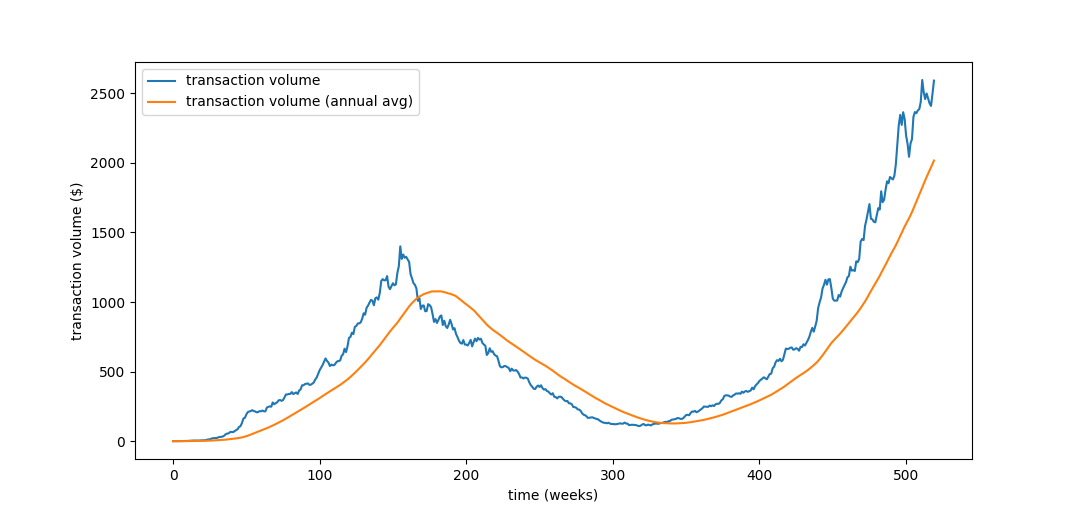
\includegraphics[scale=0.57]{/Users/nicholas/Dropbox/terra/graphs/mining_rewards_graphs/WP/TV}

\end{adjustbox}

\begin{adjustbox}{center}

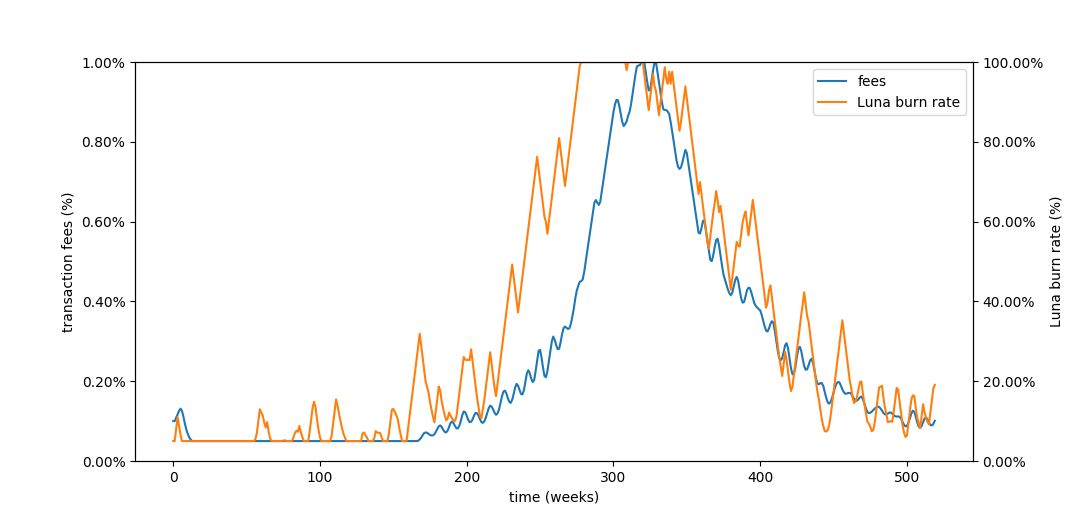
\includegraphics[scale=0.57]{/Users/nicholas/Dropbox/terra/graphs/mining_rewards_graphs/WP/fw}

\end{adjustbox}

\begin{adjustbox}{center}

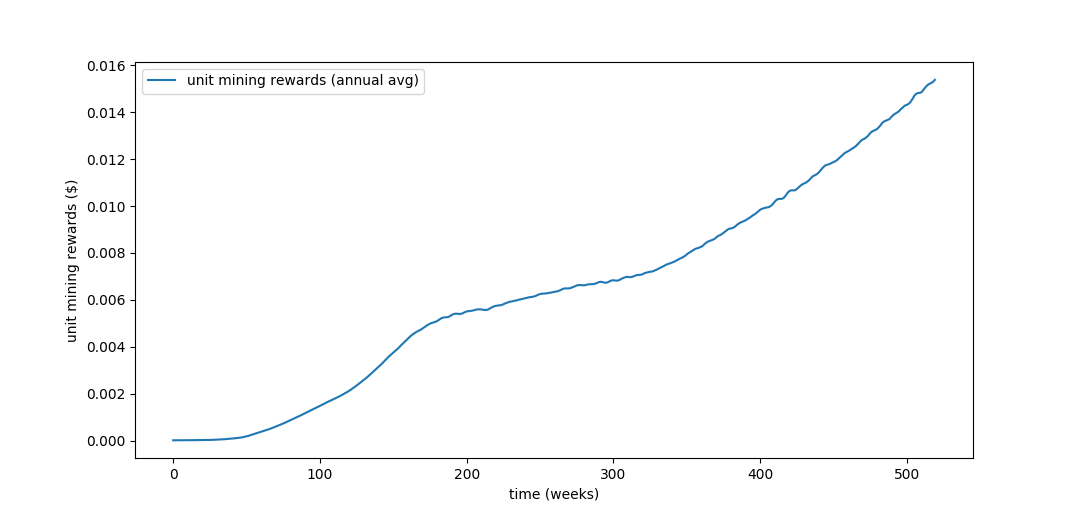
\includegraphics[scale=0.57]{/Users/nicholas/Dropbox/terra/graphs/mining_rewards_graphs/WP/MRL}

\end{adjustbox}

The first graph shows simulated weekly \textbf{transaction volume}
and its annual moving average. Transaction volume can be thought of
as the GDP of the Terra economy. The economy experiences rapid growth
followed by a severe multi-year recession that wipes out 93\% of GDP
over 3 years and requires 6 years for full recovery. This scenario
is a stern test -- if it were describing the price of Bitcoin it
would be by far the longest bear market in its history and tied for
worst in terms of drawdown (equal to the 93\% drop between June and
November 2011). While we think that Terra's adoption-driven demand
will be far more stable than Bitcoin's speculation-driven demand,
the stability mechanism has been designed to confidently withstand
Bitcoin-level volatility.

The second graph shows \textbf{transaction fees and the Luna burn
rate}, the two levers used by the protocol to smooth out fluctuations
in unit mining rewards. We observe that both move \emph{opposite}
to the direction of the economy (which is also the default direction
of unit mining rewards).

The third graph shows the annual moving average of \textbf{unit mining
rewards. }The growth target we have set in this example is 15\% annually.
As was designed, unit mining rewards experience steady growth with
low volatility, unpurturbed by the cycles in Terra's GDP. The adjustments
in fees and the Luna burn rate have successfully absorbed the expected
volatility in unit mining rewards and created predictable growth.
This is achieved with fees that average less than 0.5\% (with a momentary
peak at the 1\% maximum) and a Luna burn rate that averages roughly
50\% (meaning that on average 50\% of seigniorage is granted to the
Treasury).

Stable demand for mining is a core requirement for the security and
stability of Terra. Unit mining rewards are the primary consideration
and the biggest source of risk for miners. They are by default highly
cyclical, hence highly uncertain. Reducing that uncertainty in the
face of volatile conditions is the key to stable mining demand. We
have outlined a simple mechanism that uses transaction fees and Luna
burn as levers to achieve this, and demonstrated its effectiveness
in the most severe economic conditions.

\section{Growth-driven fiscal policy}

Despite their enormous potential, smart contracts have faced roadblocks
in adoption due to the price volatility of their underlying currency.
Price volatility makes smart contracts unusable for most mainstream
financial applications, as most users are accustomed to valuing determinate
payouts in insurance, credit, mortgage, and payroll. Terra will offer
a stable dApp platform oriented to building financial applications
that use Terra as their underlying currency, thus allowing smart contracts
to mature into a useful infrastructure for mainstream businesses.
Terra Platform DApps will help to drive growth and stabilize the Terra
family of currencies by diversifying its use cases. In this section
we discuss how the protocol subsidizes the growth of the more successful
applications through its growth-driven fiscal policy.

National governments use expansionary fiscal spending with the objective
of stimulating growth. The hope of fiscal spending is that the economic
activity instigated by the original spending results in a feedback
loop that grows the economy more than the amount of money spent in
the initial stimulus. This concept is captured by the spending multiplier
--- how many dollars of economic activity does one dollar of fiscal
spending generate? The spending multiplier increases with the marginal
propensity to consume, meaning that the effectiveness of the expansionary
stimulus is directly related to how likely economic agents are to
increase their spending.

In a previous section, we discussed how Terra seigniorage is directed
to both miner rewards and the Treasury. At this point, it is worth
describing how exactly the Treasury implements Terra's fiscal spending
policy, with its core mandate being to stimulate Terra's growth while
ensuring its stability. In this manner, Terra achieves greater efficiency
by returning seigniorage not allocated for stability back to its users.

The Treasury's main focus is the allocation of resources derived from
seigniorage to decentralized applications (dApp). To receive seigniorage
from the Treasury, a dApp needs to register for consideration as an
entity that operates on the Terra network. dApps are eligible for
funding depending on their economic activity and use of funding.

The funding procedure for a dApp works as follows: 
\begin{itemize}
\item A dApp applies for an account with the Treasury; the application includes
metadata such as the Title, a url leading to a detailed page regarding
the use of funding, the wallet address of the applicant, as well as
auditing and governance procedures. 
\item At regular voting intervals, Luna validators vote to accept or reject
new dApp applications for Treasury accounts. The net number of votes
(yes votes minus no votes) needs to exceed 1/3 of total available
validator power for an application to be accepted. 
\item Luna validators can exercise control over which dApps may open accounts
with the Treasury. The funding itself is determined by validator voting
for each funding period in accordance with a weight that is assigned
to each dApp. This allows the Treasury to prioritize dApps that earn
the most funding. 
\item At each voting session, Luna validators have the right to request
that a dApp be blacklisted, for example because it behaves dishonestly
or fails to account for its use of Treasury funds. Again, the net
number of votes (yes votes minus no votes) needs to exceed 1/3 of
total available validator power for the blacklist to be enforced.
A blacklisted dApp loses access to its Treasury account and is no
longer eligible for funding. 
\end{itemize}
The motivation behind assigning funding weights to dApps is to maximize
the impact of the stimulus on the economy by rewarding the dApps that
are more likely to have a positive effect on the economy. The Treasury
uses two criteria to determine spending allocations: (1) \textbf{robust
economic activity} and (2) \textbf{efficient use of funding}. dApps
with a strong track record of adoption receive support for their continued
success, and dApps that have grown relative to their funding are rewarded
with more seigniorage, as they have a successful track record of efficiently
using their resources.

Those two criteria are combined into a single weight which determines
the relative funding that dApps receive from the aggregate funding
pool. For instance, a dApp with a weight of 2 would receive twice
the amount of funding of a dApp with a weight of 1.

We lay out the funding weight equation, followed by a detailed explanation
of all the parts: For a time period t, let $TV_{t}$ be a dApp's transaction
volume and $F_{t}$ be the Treasury funding received. Then, the protocol
determines the funding weight $w_{t}$ for the period as follows:

\[
w_{t}=\left(1-\lambda\right)TV_{t}^{*}+\lambda\frac{\Delta TV_{t}^{*}}{F_{t-1}^{*}}
\]

The notation {*} denotes a moving average, so $TV_{t}^{*}$ would
be the moving average of transaction volume leading up to time period
t, while $\Delta TV_{t}^{*}$ would be a difference of moving averages
of different lengths leading up to time period t. One might make the
averaging window quarterly for example. Finally, the funding weights
among all dApps are scaled to sum to 1.
\begin{itemize}
\item \textbf{The first term} is proportional to $TV_{t}^{*}$, the average
transaction volume generated by the dApp in the recent past. This
is an indicator of the dApp's \textbf{economic activity}, or more
simply the size of its micro-economy. 
\item \textbf{The second term} is proportional to $\Delta TV*_{t}/F*_{t}-1$.
The numerator describes the trend in transaction volume --- it is
the difference between a more and a less recent average. When positive,
it means that the transaction volume is following an upward trajectory
and vice versa. The denominator is the average funding amount received
by the dApp in the recent past, up to and including the previous period.
So the second term describes how economic activity is changing relative
to past funding. Overall, larger values of this ratio capture instances
where the dApp is fast-growing for each dollar of funding it has received.
This is in fact the spending multiplier of the funding program, a
prime indicator of \textbf{funding efficiency}. 
\item The parameter \textgreek{l} is used to determine the relative importance
of economic activity and funding efficiency. If it is set equal to
1/2 then the two terms would have equal contribution. By decreasing
the value of \textgreek{l}, the protocol can favor more heavily dApps
with larger economies. Conversely, by increasing the value of \textgreek{l}
the protocol can favor dApps that are using funding with high efficiency,
for example by growing fast with little funding, even if they are
smaller in size.
\end{itemize}
An important advantage of distributing funding in a programmatic way
is that it is simpler, objective, transparent and streamlined compared
to open-ended voting systems. In fact, compared to decentralized voting
systems, it is more predictable, because the inputs used to compute
the funding weights are transparent and slow moving. Furthermore,
this system requires less trust in Luna validators, given that the
only authority they are vested with is determining whether or not
a dApp is honest and makes legitimate use of funding.

Overall, the objective of Terra governance is simple: fund the organizations
and proposals with the highest net impact on the economy. This will
include dApps solving real problems for users, increasing Terra's
adoption and as a result increasing the GDP of the Terra economy.

\section{Conclusion}

We have presented Terra, a stable digital currency that is designed
to complement both existing fiat and cryptocurrencies as a way to
transact and store value. The protocol adjusts the supply of Terra
in response to changes in demand to keep its price stable. This is
achieved using Luna, the mining token whose stable rewards are designed
to absorb volatility from changing economic cycles. Terra also achieves
efficient adoption by returning seigniorage not invested in stability
back to its users. Its transparent and democratic distribution mechanism
gives dApps the power to attract and retain users by tapping into
Terra's economic growth.

If Bitcoin's contribution to cryptocurrency was immutability, and
Ethereum expressivity, our value-add will be usability. The potential
applications of Terra are immense. Immediately, we foresee Terra being
used as a medium-of-exchange in online payments, allowing people to
transact freely at a fraction of the fees charged by other payment
methods. As the world starts to become more and more decentralized,
we see Terra being used as a dApp platform where price-stable token
economies are built on Terra. Terra is looking to become the first
usable currency and stability platform on the blockchain, unlocking
the power of decentralization for mainstream users, merchants, and
developers.

\noindent {\small{}{}\newpage}\textbf{\small{}{}References }{\small\par}

\noindent {\small{}{}Liu, Yukun and Tsyvinski, Aleh, Risks and Returns
of Cryptocurrency (August 2018). NBER Working Paper No. w24877. Available
at https://ssrn.com/abstract=3226806. }{\small\par}

\noindent {\small{}{}Makarov, Igor and Schoar, Antoinette, Trading
and Arbitrage in Cryptocurrency Markets (April 30, 2018). Available
at SSRN: https://ssrn.com/abstract=3171204. }{\small\par}

\noindent {\small{}{}Kereiakes, Evan, Rationale for Including Multiple
Fiat Currencies in Terra's Peg (November 2018). Available at https://medium.com/terra-money/rationale-for-including-multiple-fiat-currencies-in-terras-peg-1ea9eae9de2a }{\small\par}

\noindent {\small{}{}Taylor, John B. (1993). \textquotedbl Discretion
versus Policy Rules in Practice.\textquotedbl{} Carnegie-Rochester
Conference Series on Public Policy. 39: 195--214. }{\small\par}

 
\end{document}
